\chapter{“香山”处理器虚拟化扩展的设计}

% 1. 调研其他项目
% 2. 本文的优点
% 3. 如何组织组织自己的工作,凸显自己的逆天、遇到困难多、提出的想法好。

\section{特权相关部件设计扩展}
实现虚拟化扩展的特权相关部分,
涉及到处理器核的主要修改如图\ref{fig:xs-h-ext-priv}深绿色的部分所示,
包括前端的取指单元、指令缓冲、指令队列、解码器,
后端的控制状态寄存器执行单元、栅栏指令执行单元、访存流水线,访存队列。
尽管包括较多的流水线和功能模块,但大体可以分为特权控制和特权指令两个部分。

\begin{figure}[htbp]
    \centering
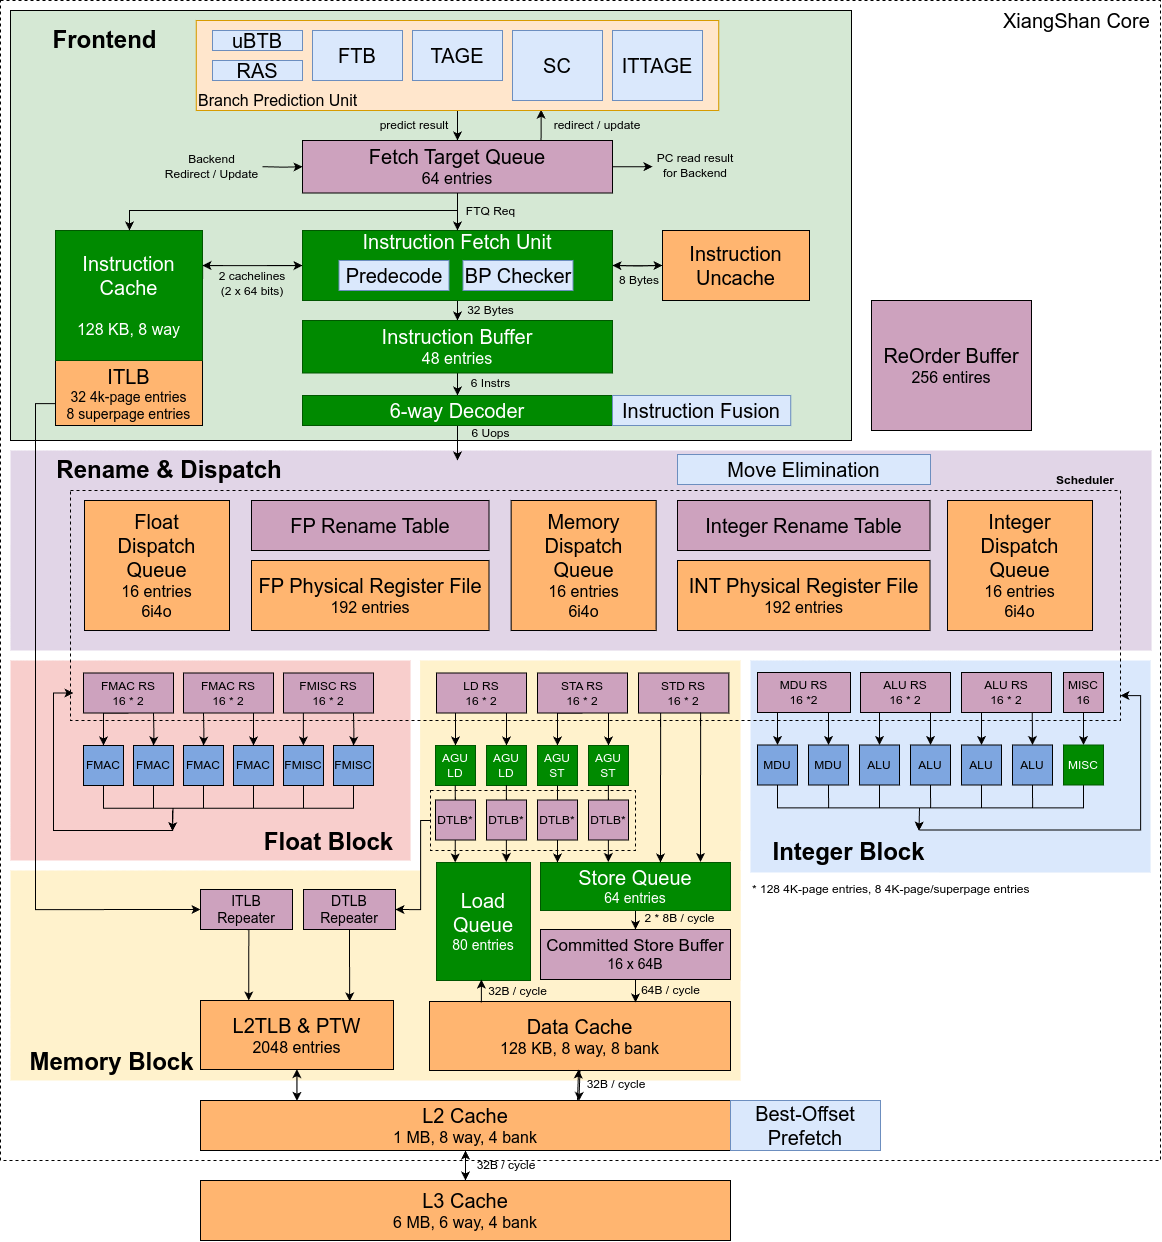
\includegraphics[scale=0.3]{xs-h-ext-priv.png}
    \caption{特权相关部件扩展涉及到的“南湖”的流水线}
    \label{fig:xs-h-ext-priv}
\end{figure}

\paragraph{特权控制}
该部分修改主要集中在控制状态寄存器执行单元中,包括特权级别的新增和控制状态寄存器的扩展。

\subparagraph{特权级别}
通过在硬件中添加虚拟位到原始的特权级别中,代表处理器是否开启了虚拟化,
用于区分虚拟机管理模式与虚拟监管模式、虚拟用户模式和普通用户模式。
同时,一级页表缓冲、地址翻译引擎、解码单元等模块需要当前的虚拟化模式信息,
所以需要在CSR执行单元的输出信号中添加虚拟化模式信号,将虚拟化模式信息传递到其他模块。

\subparagraph{控制状态寄存器}
需要添加的部分主要包括虚拟机管理模式的、虚拟监管模式的控制状态寄存器。
其中,虚拟管理模式下的相关CSR实现较为单一,仅需按照手册添加对应的功能:
包括配置处理器捕获敏感指令的能力,虚拟机管理模式的中断委托、使能、挂起等。
值得一提的是虚拟监管模式下的控制状态寄存器的读写处理。
根据当前特权级别中的虚拟位是否置起:控制状态寄存器的读写指令传入的寄存器地址可
以代表虚拟监管模式下的寄存器(例如stvec),
也可以代表对应的虚拟机管理模式下的寄存器(例如vstvec)。
所以需要使用当前特权级等信息对地址再映射。
此外,在虚拟机管理模式的CSR中,存在vsip和vsie这两个特殊的寄存器,
用于控制虚拟机中断的挂起和使能。
在实现方式上,不存在实际的物理寄存器,而是对mip和mie两个寄存器的切片映射。
例如,软件在读写,认为中断位为1、5、9位,但实际上是写入mip和mie的
2、6、10位,所以需要对读写数据进行特殊处理,根据读写寄存器是否是vsip
和vsie,来决定是否对数据进行移位操作。

\paragraph{特权指令}
特权指令均和第二阶段地址翻译相关,包括用于第二阶段页表的屏障指令HFENCE.VVMA/GVMA、
在未开启虚拟化模式时启用第二阶段地址翻译的访存指令HLV.width, HLVX.HU/WU, HSV.width。
作为特权指令,只能在非虚拟化模式下执行。
如果尝试在虚拟化模式下执行,则引发虚拟化指令异常,给控制流的异常向量信号的对应位赋值。
根据流水线由前至后的顺序,最先需要修改的是译码单元、派发、保留站部分。
这些部分因为Chisel高级语言的特性以及“香山”项目的良好基础架构,
仅需将指令添加到表格中,并指出所需派发到的保留站、功能单元的操作符等即可。
HFENCE.VVMA/GVMA指令需要交由屏障指令执行单元,访存相关指令交由内存访问流水线执行。
虚拟化访存指令是虚拟机管理系统访问虚拟机内存的手段,该类指令会启用两阶段地址翻译,
并且执行和虚拟机状态下一样的地址转换和类型检查。
该类指令主要在访存流水线中执行,并且执行的过程如表\ref{tab:h-ls}所示,
受多个控制状态寄存器影响。
除了对应的特权保护相关部分,需要在向一级页表缓冲发送地址翻译请求的时候,
指定是两阶段地址翻译,添加相关的控制状态寄存器的信息,例如ASID和VMID等。
虚拟化内存屏障指令则是复用了原有的内存屏障数据通路的状态机,
都是先等待写缓冲(Store Buffer)的清空,之后再向页表缓冲发送无效化的请求。
修改主要是对页表缓冲发送的无效化请求进行,在其中添加虚拟化内存屏障指令相关的字段。

\begin{table}
    \centering
    \caption{控制状态寄存器字段对虚拟化访存指令执行的影响}
    \begin{tabular}{cc}
        \toprule
        CSR字段        & 对虚拟化访存指令的影响      \\
        \midrule
        hstatus.hu   & 用户模式下能否执行虚拟化访存指令 \\
        hstatus.spvp & 控制虚拟化访存指令的执行特权级  \\
        sstatus.mxr  & 第二阶段的可执行权限页表是否可读 \\
        vstatus.mxr  & 第一阶段的可执行权限页表是否可读 \\
        \bottomrule
    \end{tabular}
    \label{tab:h-ls}
\end{table}

\section{内存管理单元设计扩展}
添加虚拟化扩展后的内存管理单元如图\ref{fig:after-mmu}所示,
主要的变化包括:添加第二阶段地址翻译单元、扩展一级页表缓存以支持两阶段地址翻译、
扩展二级页表缓存使其被两阶段页表共享、适配页目录翻译单元和叶表项翻译单元。
此外,该该部分还会分析Rocket Chip和CVA6,
目前两个实现了虚拟化扩展的开源RISC-V处理器的的虚拟内存管理单元和“香山”内存管理单元的优缺点。

\begin{figure}[htbp]
\centering
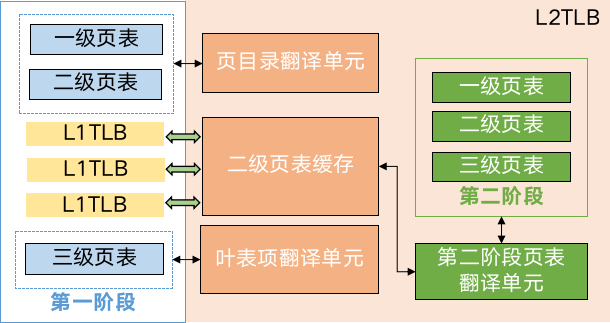
\includegraphics[scale=0.8]{after-mmu.png}
\caption{“香山”处理器添加虚拟化扩展后的内存管理单元}
\label{fig:after-mmu}
\end{figure}

\paragraph{第二阶段地址翻译单元}
该模块负责将虚拟机物理地址翻译成主机物理地址,需要多次访问内存解析页表。
实现方式采用朴素的阻塞状态机,一次仅处理一个请求。
但是对外暴露的端口采用的是Ready-Valid解耦形式的设计,
因此可以在不改变外部连接的情况下优化内部设计,以实现流水线或者并发。
在外部,和该模块直接相连的是二级页表缓存。
当向二级页表缓存查询第二阶段地址翻译不命中时,二级页表缓存会对该模块发起翻译请求。
翻译的结果会被缓存到二级页表缓存中。该模块相对于二级页表缓存,作为一个替换模块被使用。
因此,在初期使用阻塞的朴素实现,既可以观察二级页表缓存的缓存能力,也能够减少模块复杂度保证正确性。

\paragraph{二级页表缓存}
该模块是L2 TLB的中心,负责直接回复一级页表缓存的地址翻译请求。
在虚拟化扩展下,一级页表缓存会发送仅第一阶段、仅第二阶段和两阶段联合的三种类型的地址翻译请求。
但在原始架构下只实现了回复仅第一阶段的地址翻译的功能,
为了尽可能减少修改、同时尽可能快地回复三种类型的请求,通过在缓存条目中添加新的标志位区分页表的阶段。
具体而言,二级页表缓存中的所有缓存条目要么是仅第一阶段页表,要么是仅第二阶段页表,
和一级页表缓存条目完全不相同,不存在两阶段联合的缓存条目。
在这种设计下,可以快速的响应仅第一阶段的请求和仅第二阶段的请求。
对于两阶段联合的请求,则需要先向二级页表缓存发起第一阶段地址翻译请求,同时将请求缓存在寄存器。
得到第一阶段的翻译结果,即虚拟机物理地址后,再对二级页表缓存发起第二阶段地址翻译请求得到主机物理地址。
诚然,两阶段联合翻译时间是单阶段翻译时间的两倍,
但通过将二级页表缓存流水线化、使用不命中队列等方法,能够在一定程度上减少繁忙时期的查询开销。

虚拟化扩展下新增了HFENCE.VVMA和HFENCE.GVMA两条关于虚拟内存同步指令指令。
该指令用于在虚拟机管理模式下,同步内存中的两阶段的页表数据结构。
对于二级页表缓存,需要在执行指令时的将对应的,必须要无效化的条目无效化,
比如地址相同的或者是虚拟机编号(VMID)、进程编号(ASID)相同的条目。
仅无效化必要的条目可以称作精确无效化,但实现的复杂度较高。
也可以无效化全部条目保证以正确性和简便性,但是对效率较低。
另一方面,由于各级页表的不同数据分别存储在寄存器或者静态随机访问存储器(SRAM)
由于SRAM的同步读特性,精确无效化的实现难度相对寄存器言较高。
此外,各阶段各级页表的复用频率各不相同,需要在效率和实现复杂度中找到一个折中。
在目前的设计中,各阶段的各级页表缓存的有效位(valid)、全局位(global)和虚拟位(hypervisor)均使用寄存器实现。
因此均可简易地实现仅第一阶段或者第二阶段的页表无效化,
这种设计能够满足两种HFENCE指令的较低要求,即区分两阶段的页表。
进一步,对于VMID和ASID的精确无效化,仅在一级页表进行了实现。
因为其采用16项全相连的寄存器存储实现,可以较为快速地读取并计算需要无效化的条目。
而二级页表和三级页表的数据位均存储在SRAM中,难以实现快速的、简易的无效化。
最后,关于指定地址的精确无效化,只实现了第三级页表的大致的无效化。
则是使用指定地址的索引部分(index)查找存储器对应的条目,并将其无效化。
即不论标识部分(tag)是否相同,只要index相同则被无效化。
这种实现方式完全不需要读取SRAM,实现复杂度不高。
尽管会造成一定的性能损失,但是最多会将nWays(缓存路数)个不需要被无效化的条目无效,
是一个可接受的折中。

\paragraph{第一阶段地址翻译单元}
在虚拟化扩展下,第一阶段地址翻译单元仍然负责第一阶段的地址翻译。
最主要的修改是在每次访存前将客户机物理地址翻译成主机物理地址。
实现方式是通过增加自动机的状态,在发起访存请求前先对外发起第二阶段的地址翻译。
值得一提的是外界对第一阶段地址翻译单元发起的第二阶段地址翻译请求的回应方式。
如果直接发送到第二阶段地址翻译单元,无法充分利用二级页表缓存中的虚拟页条目。
因此请求会在仲裁后被先转发到二级页表缓存,如果不命中再由第二阶段地址翻译单元进行访存。
在这种方式下,一次命中可以减少3次内存访问,能够较为有效的提高翻译速度和二级页表缓存的利用率。

另一方面,第一阶段地址翻译单元由页目录和叶表项两个翻译单元组成,
分别负责第一阶段的前两级和最后一级的页表翻译。
两个模块虽然功能相似,实则具有不同的特点,在虚拟化扩展下也有不同的修改。
\subparagraph{页目录翻译单元}
主要的功能是作为二级页表缓存的替换单元,负责直接承接二级页表缓存的的不命中请求。
再根据请求的阶段和级数,转发给自己的自动机、叶表项翻译单元或者是进行第二级地址翻译。
因此实现上主要是体现一个灵活实现和功能接口丰富,接受所有可能的L2 TLB查询结果。
例如,在二级页表缓存的查询结果是第一阶段页表翻译直接命中页节点,但是第二阶段未命中。
此时将请求缓存,并发起第二阶段地址翻译,等待返回。
在二级页表查询结果是第一阶段页表翻译只命中了页目录,此时需要启动自己的自动机。
先发起第二阶翻译请求,将页目录的客户机物理地址翻译成主机物理地址;在根据返回结果判断权限、组合下一级页表的地址。
重复该过程直到找到叶表项的地址,之后把请求转发给叶表项翻译单元。
\subparagraph{叶表项翻译单元}
负责接收来自二级页表缓存和页目录翻译单元的叶表项翻译请求。
请求的频率必然高于页目录翻译单元,因此在实现上主要追求高并发和快速。
优化的切入点在于叶表项总是连续的,可以使用猝发访存,一次获取多个相邻的叶表项。
在硬件实现上,存在多个缓存槽,因此叶表项翻译单元可以非阻塞的接收多个请求。
每此接收新请求,分配缓存槽的时候,会根据请求的虚拟机物理地址判断是是否位于同一缓存行,
能否在同一个猝发访存中得到结果。如果可以,新请求会使用等待槽编号记录旧请求的缓存槽编号。
当访存返回时,对所有等待槽编号与该访存的缓存槽编号相同的缓存槽的状态进行转换。
代表访存结果已经返回,之后由出队逻辑将所有已完成的缓存槽逐个出队。
然而,在虚拟化扩展下,访存返回的仅仅是虚拟机物理地址,
还需要再经过一次第二阶段地址翻译将其翻译成主机物理地址。
现阶段的实现是使用自动机第二阶段翻译请求向外发送,
该请求会与页目录翻译单元的第二阶段请求进行仲裁后会被发送到二级页表缓存查询。
叶表项翻译单元不需要理解外界如何处理其第二阶段地址翻译请求,只需要等待翻译结果并返回即可。
尽管这是一个不太有效率的做法,但是没有破坏原本的第一阶段叶表项的高吞吐量。

\paragraph{一级页表缓存}
一级页表缓存作为分布式的小容量全相连页表缓存,
分布式地布线在取指单元(IFU)和访存单元(Memory Block),能够减少时序压力。
主要负责通过一个时钟周期的时间,快速地将虚拟机虚拟地址转换为主机物理地址。
为了在支持快速地两阶段地址翻译的同时,兼容仅第一阶段的地址翻译,
需要在缓存条目中添加虚拟化位和虚拟机标识。
此外,一个缓存条目还存储了多个权限阶段等信息相同的有效的物理地址。
即可以根据虚拟地址的低位标识(tag)来索引不同的物理地址。
该优化的想法来源于连续的虚拟页的权限和异常信息可能具有局部性,
而且来自二级页表缓存的充填数据是以缓存块的形式返回多个翻译结果。
实现则是通过使用一组寄存器,按照虚拟地址的低3位标识存储物理地址的低3位标识。
较少的组数,可以保证布线的负担不会太大,对于特殊情况的优化效果也是明显的。

虚拟化扩展在异常方面也需要一级页表缓存提供额外的支持。
即虚拟机缺页异常,表示在进行第二阶段地址翻译是触发了缺页。
在实现方面,一级页表缓存仅保存是否发生了相关异常,而异常所对应的虚拟机物理地址,由于容量原因则不保存在数据表项中。
需要在响应请求时判断:如果命中的页表条目发生了虚拟机缺页异常,
则返回不命中,同时向二级页表缓发起翻译请求,直到返回虚拟机物理地址后,一级页表缓存才会响应命中。
鉴于虚拟机缺页异常发生频率较低,这种以时间换面积开销的解决方案是可接受的。

\section{设计扩展正确性评测}
为了验证虚拟化扩展实现的正确性,
本文使用riscv-hyp-test\cite{itco2022rocket}进行验证。
这是一个开源的,针对RISC-V的虚拟化扩展的测试,是一个小型的裸机程序。
最初是是Rocket Chip在开发虚拟化时编写的,用于加速开发的简易测试。
如表\ref{tab:hyp-test}所示,
hyp-test包括特权指令、虚拟内存、异常中断三个方面,每个方面都有若干个小测试。

\begin{table}
    \centering
    \caption{riscv-hyp-test的测试和功能}
    \begin{tabular}{ccc}
        \toprule
        类别   & 基准测试                          & 测试目标             \\
        \midrule
        特权指令 & wfi exception tests           & VS和HS下执行wfi指令    \\
        特权指令 & hfence test                   & HS的页表同步指令        \\
        特权指令 & virtual instruction           & VS下执行hyper特权指令   \\
        虚拟内存 & two stage translation         & VS下通过两级页表翻译访问内存  \\
        虚拟内存 & second stage only translation & HS下仅第二级页表翻译访问内存  \\
        虚拟内存 & m and hs using vs access      & HS下通过两级页表翻译访问内存  \\
        异常中断 & interrupt tests               & HS下挂起虚拟机中断       \\
        异常中断 & check xip regs                & HS下中断委托、挂起寄存器    \\
        异常中断 & tinst tests                   & HS和VS异常需写入特定的CSR \\
        \bottomrule
    \end{tabular}
    \label{tab:hyp-test}
\end{table}

测试的运行环境是开源的逻辑软件仿真工具verilator。
由于该测试程序不需要任何引导程序或者操作系统,
把测试程序的二进制文件放入仿真内存的处理器复位时跳转的地址,即可正常执行。
采用软件逻辑仿真的是因为是测试程序足够小,能够在几分钟内快速的完成。
此外,逻辑仿真软件能够获取波形文件,对硬件调试有巨大的帮助。
然而,完全运行测试仍然需要数万个时钟周期,无法精确地定位出错现场。
因此还使用了差分测试的方法来快速地定位错误时刻。
通过使用RISC-V处理器模拟器NEMU,一个软件实现的处理器金标准。
在每条指令执行的时候,对比“香山”和金标准的所有架构处理器。
可以将错误发生现场缩短在一条指令的执行周期内。
在以上工具的帮助下,通过了每个方面的测试,运行结果如图\ref{fig:hyp-test}所示。

\begin{figure}[htbp]
    \centering
    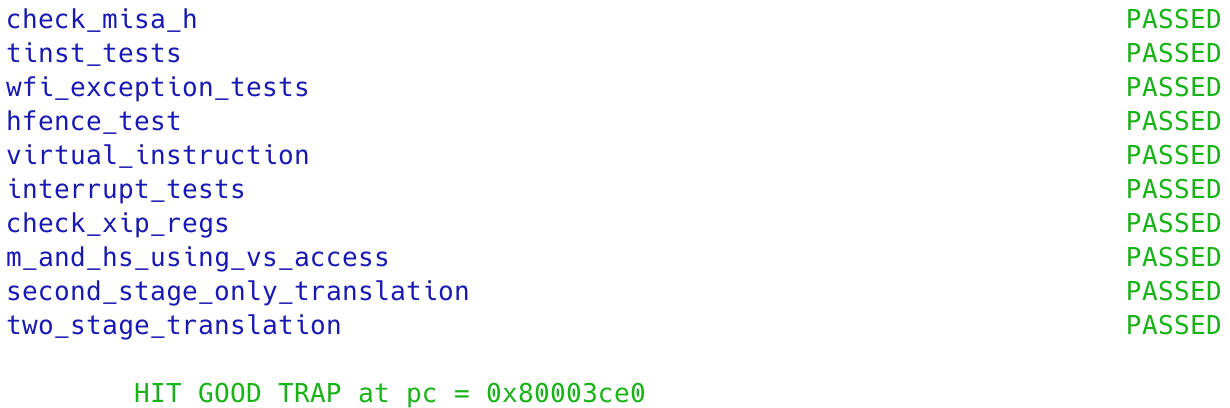
\includegraphics[scale=0.45]{hyp-test.png}
    \caption{在差分测试框架中运行hyp-test结果}
    \label{fig:hyp-test}
\end{figure}

\section{本章小结}
本章介绍“香山”处理器的“南湖”架构的虚拟化扩展的硬件实现。
虚拟化扩展的修改,可以分为特权相关部件和内存管理单元两部分。
在完成了硬件扩展后,使用一个专用于RISC-V虚拟化扩展的小型裸机程序测试,测试功能的正确性。